\documentclass[12pt, twoside]{article}
\usepackage[letterpaper, margin=1in, headsep=0.2in]{geometry}
\setlength{\headheight}{0.6in}
%\usepackage[english]{babel}
\usepackage[utf8]{inputenc}
\usepackage{microtype}
\usepackage{amsmath}
\usepackage{amssymb}
%\usepackage{amsfonts}
\usepackage{siunitx} %units in math. eg 20\milli\meter
\usepackage{yhmath} % for arcs, overparenth command
\usepackage{tikz} %graphics
\usetikzlibrary{quotes, angles}
\usepackage{graphicx} %consider setting \graphicspath{{images/}}
\usepackage{parskip} %no paragraph indent
\usepackage{enumitem}
\usepackage{multicol}
\usepackage{venndiagram}

\usepackage{fancyhdr}
\pagestyle{fancy}
\fancyhf{}
\renewcommand{\headrulewidth}{0pt} % disable the underline of the header
\raggedbottom
\hfuzz=2mm %suppresses overfull box warnings

\usepackage{hyperref}

\fancyhead[LE]{\thepage}
\fancyhead[RO]{\thepage \\ Name: \hspace{4cm} \,\\}
\fancyhead[LO]{BECA / Dr. Huson / Geometry\\*  Unit 5: Pythagorean theorem\\* 29 November 2022}

\begin{document}

\subsubsection*{5.3 Classwork: Distance formula}
\begin{enumerate}
\item Do Now: Use a centimeter ruler to measure the triangle side lengths.
\begin{flushright}
    \begin{tikzpicture}[scale=1]
    \node at (4,3)[above left]{$c$};
    \node at (8,3)[right]{6 cm};
    \node at (4,0)[below]{8 cm};
    \draw [thick] (0, 0)--(8, 0)--(8, 6)--cycle;
    \draw [dashed] (8,0)++(-0.4,0)-- ++(0,0.4)-- +(0.4,0);
    \end{tikzpicture}
\end{flushright}

    
\item What is the length of $\overline{PQ}$ if $p(3,1)$ and $Q(9,1)$? \vspace{2cm}
    
Note: The formula for distance is $\displaystyle d=\sqrt{(x_2-x_1)^2+(y_2-y_1)^2}$

\item Graph and label $\triangle ABC$. Calculate the lengths of its sides. $A(1,2)$, $B(9,8)$, $C(9,2)$.
    \begin{enumerate}
        \begin{multicols}{2}
        \item   $AC=$ \vspace{1.cm}
        \item   $BC=$ \vspace{1.cm}
        \item   $AB=$ \vspace{3cm}
        \begin{center}
            \begin{tikzpicture}[scale=.635]
            \draw [help lines] (0,0) grid (10,9);
            \draw [thick, ->] (0,0) -- (10.4,0) node [below right] {$x$};
            \draw [thick, ->] (0,0)--(0,9.4) node [right] {$y$};
            \foreach \x in {1,...,10}
            \draw[shift={(\x,0)}] (0pt,-3pt)--(0pt,3pt) node[below=5pt] {$\x$};
            \foreach \y in {1,...,9}
            \draw[shift={(0,\y)}] (-3pt,0pt)--(3pt,0pt) node[left=5pt] {$\y$};
            \end{tikzpicture}
            \end{center}
        \end{multicols}
    \end{enumerate}

\newpage
\item Graph and label $\triangle ABC$. Calculate the lengths of its sides. $A(0,0)$, $B(12,5)$, $C(12,0)$.
\begin{flushleft}
    \begin{tikzpicture}[scale=.635]
    \draw [help lines] (0,0) grid (13,8);
    \draw [thick, ->] (0,0) -- (13.4,0) node [below right] {$x$};
    \draw [thick, ->] (0,0)--(0,8.4) node [right] {$y$};
    \foreach \x in {1,...,13}
    \draw[shift={(\x,0)}] (0pt,-3pt)--(0pt,3pt) node[below=5pt] {$\x$};
    \foreach \y in {1,...,8}
    \draw[shift={(0,\y)}] (-3pt,0pt)--(3pt,0pt) node[left=5pt] {$\y$};
    \end{tikzpicture}
\end{flushleft}
    
\item Graph and label $\triangle CAT$. Calculate the lengths of its sides. $C(2,1)$, $A(12,6)$, $T(12,1)$. Leave the result as a (simplified) radical if necessary, not a decimal approximation.
\begin{flushleft}
\begin{tikzpicture}[scale=.5]
    \draw [help lines] (0,0) grid (13,8);
    \draw [thick, ->] (0,0) -- (13.4,0) node [below right] {$x$};
    \draw [thick, ->] (0,0)--(0,8.4) node [right] {$y$};
    \foreach \x in {1,...,13}
    \draw[shift={(\x,0)}] (0pt,-3pt)--(0pt,3pt) node[below=5pt] {$\x$};
    \foreach \y in {1,...,8}
    \draw[shift={(0,\y)}] (-3pt,0pt)--(3pt,0pt) node[left=5pt] {$\y$};
\end{tikzpicture} \vspace{1cm}
\end{flushleft}

\item The base of a right triangle is 4 centimeters long and its hypotenuse is 5 cm. Find its height, $x$ cm.
\begin{flushright}
\begin{tikzpicture}[scale=1]
    \node at (2,1.5)[above left]{5};
    \node at (4,1.5)[right]{$x$};
    \node at (2,0)[below]{4};
    \draw [thick] (0, 0)--(4, 0)--(4, 3)--cycle;
    \draw [dashed] (4,0)++(-0.4,0)-- ++(0,0.4)-- +(0.4,0);
\end{tikzpicture}
\end{flushright}

\newpage
\item Graph and label $\triangle CAT$. Calculate the lengths of its sides. $C(1,2)$, $A(10,8)$, $T(10,2)$.
\begin{flushleft}
  \begin{tikzpicture}[scale=.5]
    \draw [help lines] (0,0) grid (13,8);
    \draw [thick, ->] (0,0) -- (13.4,0) node [below right] {$x$};
    \draw [thick, ->] (0,0)--(0,8.4) node [right] {$y$};
    \foreach \x in {1,...,13}
    \draw[shift={(\x,0)}] (0pt,-3pt)--(0pt,3pt) node[below=5pt] {$\x$};
    \foreach \y in {1,...,8}
    \draw[shift={(0,\y)}] (-3pt,0pt)--(3pt,0pt) node[left=5pt] {$\y$};
  \end{tikzpicture}
\end{flushleft}

\item The base of a right triangle is 8 centimeters long and its hypotenuse is 10 cm. Find its height, $x$ cm.
\begin{flushright}
  \begin{tikzpicture}[scale=1]
    \node at (2,1.5)[above left]{10};
    \node at (4,1.5)[right]{$x$};
    \node at (2,0)[below]{8};
    \draw [thick] (0, 0)--(4, 0)--(4, 3)--cycle;
    \draw [dashed] (4,0)++(-0.4,0)-- ++(0,0.4)-- +(0.4,0);
  \end{tikzpicture}
\end{flushright}


\end{enumerate}
\end{document}